% The main file of the report.
% Begin the latex document.
\documentclass[12pt, a4paper, titlepage, hyphens, utf8, title, hidelinks]{report}

% Enables the use of colour.
\usepackage{xcolor}
% Syntax high-lighting for code. Requires Python's pygments.
\usepackage{minted}
% Enables the use of umlauts and other accents.
\usepackage[utf8]{inputenc}
% Diagrams.
\usepackage{tikz}
% Settings for captions, such as sideways captions.
\usepackage{caption}
% Symbols for units, like degrees and ohms.
\usepackage{gensymb}
% Latin modern fonts - better looking than the defaults.
\usepackage{lmodern}
% Allows for columns spanning multiple rows in tables.
\usepackage{multirow}
% Better looking tables, including nicer borders.
\usepackage{booktabs}
% More math symbols.
\usepackage{amssymb}
% More math layouts, equation arrays, etc.
\usepackage{amsmath}
% More math fonts, like mathbb.
\usepackage{amsfonts}
% More theorem environments.
\usepackage{amsthm}
% More column formats for tables.
\usepackage{array}
% Adjust the sizes of box environments.
\usepackage{adjustbox}
% Better looking single quotes in verbatim and minted environments.
\usepackage{upquote}
% Better blank space decisions.
\usepackage{xspace}
% Better looking tikz trees.
\usepackage{forest}
% URLs.
\usepackage{hyperref}
% For plotting.
\usepackage{pgfplots}
% Web-related icons.
\usepackage{fontawesome}
% For including graphics.
\usepackage{graphicx}
% For the euro symbol.
\usepackage{eurosym}
% For titling appendices.
\usepackage{appendix}
% Sideways tables.
\usepackage{rotating}

% Various tikz libraries.
% For drawing mind maps.
\usetikzlibrary{mindmap}
% For adding shadows.
\usetikzlibrary{shadows}
% Extra arrows tips.
\usetikzlibrary{arrows.meta}
% Old arrows.
\usetikzlibrary{arrows}
% Automata.
\usetikzlibrary{automata}
% For more positioning options.
\usetikzlibrary{positioning}
% Creating chains of nodes on a line.
\usetikzlibrary{chains}
% Fitting node to contain set of coordinates.
\usetikzlibrary{fit}
% Extra shapes for drawing.
\usetikzlibrary{shapes}
% For markings on paths.
\usetikzlibrary{decorations.markings}
% For advanced calculations.
\usetikzlibrary{calc}

% GMIT colours.
\definecolor{gmitblue}{RGB}{20,134,225}
\definecolor{gmitred}{RGB}{220,20,60}
\definecolor{gmitgrey}{RGB}{67,67,67}

% Set the minted colour scheme.
\usemintedstyle{manni}
% Set some global minted styles.
\setminted{frame=lines,framesep=2mm,baselinestretch=1.2,fontsize=\footnotesize}

% Set the default location of images.
\graphicspath{{img/}}
% Set the depth of the table of contents.
\setcounter{tocdepth}{2}

% Begin the document.
\begin{document}

  % Include the preamble sections.
  \begin{titlepage}
  \begin{center}

    \rule{\linewidth}{0.5mm} \\[0.4cm]
    { \LARGE \bfseries A High-Quality Typesetting System Designed for the Production of Technical and Scientific Documentation \\[0.4cm] }
    
    \rule{\linewidth}{0.5mm} \\[0.8cm]
    
    \textsc{Fourth year project}\\[3cm]
    
    \noindent
    \textbf{John Doe}\\
    \textbf{Supervisor: Dr Ian McLoughlin}\\
    Department of Computer Science and Applied Physics\\
    Galway-Mayo Institute of Technology (GMIT)\\
    Galway Campus, Old Dublin Road\\
    Galway, Ireland\\[0.2cm]
    ian.mcloughlin@gmit.ie
    
    \vfill
    
    {\large \today}
    \\[1cm]
    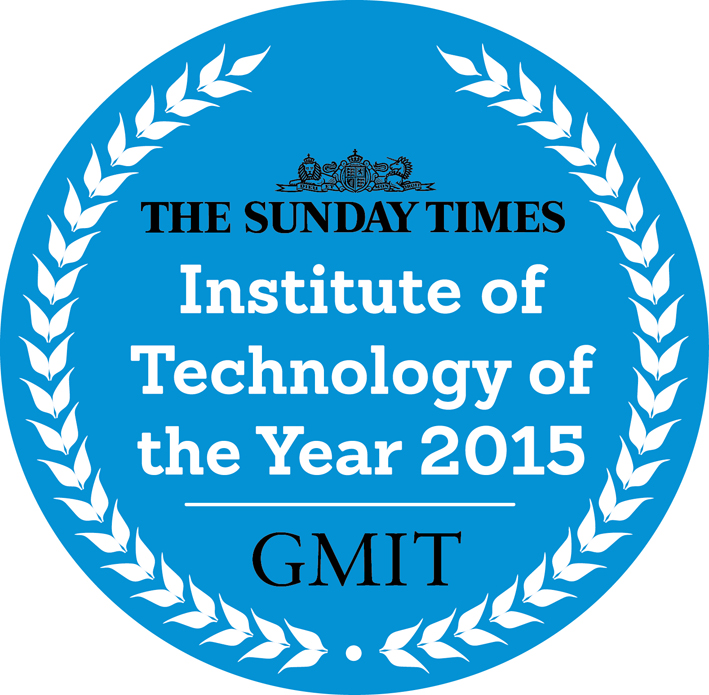
\includegraphics[width=0.35\textwidth]{gmit-sunday-times-logo-2015.jpg}
  
  \end{center}
\end{titlepage}
  \renewcommand{\abstractname}{Executive Summary}
\begin{abstract}

\noindent As part of our coursework for the B.Sc. (Honours) in Software Development at the Galway-Mayo Institute of Technology, we were required to complete a project.
\begin{description}
  \item[Review] something.
\end{description}

\end{abstract}
\newpage
  \renewcommand{\abstractname}{About the authors}
\begin{abstract}

\noindent Dr. Ian McLoughlin is a lecturer in the Department of Computer Science and Applied Physics at the Galway-Mayo Institute of Technology (GMIT) in Ireland, where he teaches modules in Algorithms, Emerging Technologies and Graph Theory, among others.
Previously he held academic positions at the Institute of Technology, Sligo, the Digital Enterprise Research Institute (now The Insight Centre for Data Analytics) at the National University of Ireland, Galway, and the Clique Research Cluster (now also Insight) at University College Dublin.

Ian has worked in industry at the Aon Centre for Innovation and Analytics in Dublin and at IBM Research in Zurich, Switzerland.
He was involved in the development of in-house web applications at IBM Research, Aon, UCD, NUIG and Stanford University.
He holds a Ph.D. in Mathematics from the National University of Ireland, Galway for which he was awarded an IRCSET scholarship.
In 2014 he was the recipient of a Fulbright TechImpact Award which he took up as a Visiting Scholar at Stanford University in California.

\end{abstract}
\newpage
  \renewcommand{\abstractname}{About GMIT}

\begin{abstract}
  GMIT~\cite{gmit:home} is a third level teaching and research institute located in the west of Ireland.
  GMIT's mission is to develop life-long learning opportunities through our teaching and research, by supporting regional development consistent with national higher education policy.
  Learning is at the core activity of the Institute, bringing students, staff and the region together to share, apply, test and create knowledge;
  GMIT aims to develop as a regional organisation with an international focus committed to the personal and professional enrichment of its students, the needs of its region, national priorities and global opportunities.
\end{abstract}
  % Create the table of contents.
  \tableofcontents
  \newpage
  % Include the main sections.
  \chapter{Introduction}
\label{chapter:introduction}

The objective of this project is to do the project.
In section \ref{chapter:platform} we discuss the platform selection.
In section \ref{chapter:conclusion} we conclude the report.
  \chapter{Review}
\label{chapter:review}

\begin{itemize}
  \item \emph{social network platform}
  \item \emph{social network software}
  \item \emph{social media platform software}
  \item \emph{social network for higher education}
  \item \emph{social network platform for higher education}
  \item \emph{white-label social network software}
\end{itemize}
  
\chapter{Platform selection}
\label{chapter:platform}

In this section we discuss the selection of a platform on which to build our prototype.
Table \ref{table:selection} is a bit big.

\begin{table}[H]
  \centering
  {\footnotesize
  \begin{tabular}{p{0.12\textwidth}p{0.25\textwidth}p{0.25\textwidth}p{0.25\textwidth}}
    \toprule
      Criterion &
      Option A &
      Option B &
      Option C \\
    \midrule
      Maintain &
      No real maintenance. &
      Easy to maintain; easy to find help. &
      Extensive technical expertise required. \\
    \midrule
      Customise &
      Generally only branding can be customised. &
      Theming and plugins provide significant customisation; lower-level customisations possible but not advised. &
      Total control over customisations, but can be onerous. \\
    \midrule
      Resilience &
      Based on the vendor's own resilience and their investment in the platform. & 
      Selection of a popular platform ensures on-going reilience. &
      Depends on all technologies used, can be volatile. \\
    \midrule
      Community &
      Depends on size of social network -- community often limited with some notable exceptions such as Facebook. &
      Large communities already established for many products. &
      Segmented community across each technology involved. \\
    \midrule
      Reliable &
      Extremely reliable, often based on Service Level Agreements. &
      Very reliable as the platforms are well established. &
      Dependent on social network maintainer's ability to ensure reliability. \\
    \bottomrule
  \end{tabular}
  }
  \caption{Selection matrix for platform}
  \label{table:selection}
\end{table}
  \chapter{Deployment}
\label{chapter:deployment}

This is where you list your deployment information.
Check out Listing \ref{listing:docker-compose}.

\begin{figure}[htp]
  \begin{minted}{yaml}
version: '3'

services:
  db:
    image: mysql:5.7
    volumes:
      - db_data:/var/lib/mysql
    restart: always
    environment:
      MYSQL_ROOT_PASSWORD: wordpress
      MYSQL_DATABASE: wordpress
      MYSQL_USER: wordpress
      MYSQL_PASSWORD: wordpress

  wordpress:
    depends_on:
      - db
    image: wordpress:latest
    volumes:
      - wp_data:/var/www/html
    ports:
      - "80:80"
    restart: always
    environment:
      WORDPRESS_DB_HOST: db:3306
      WORDPRESS_DB_PASSWORD: wordpress

volumes:
  db_data:
  wp_data:
  \end{minted}
  \caption{Docker Compose configuration file for WordPress.}
  \label{listing:docker-compose}
\end{figure}
  \chapter{Configuration}
\label{chapter:configuration}

See Figure \ref{figure:example}.

\begin{figure}[htp]
  \centering
  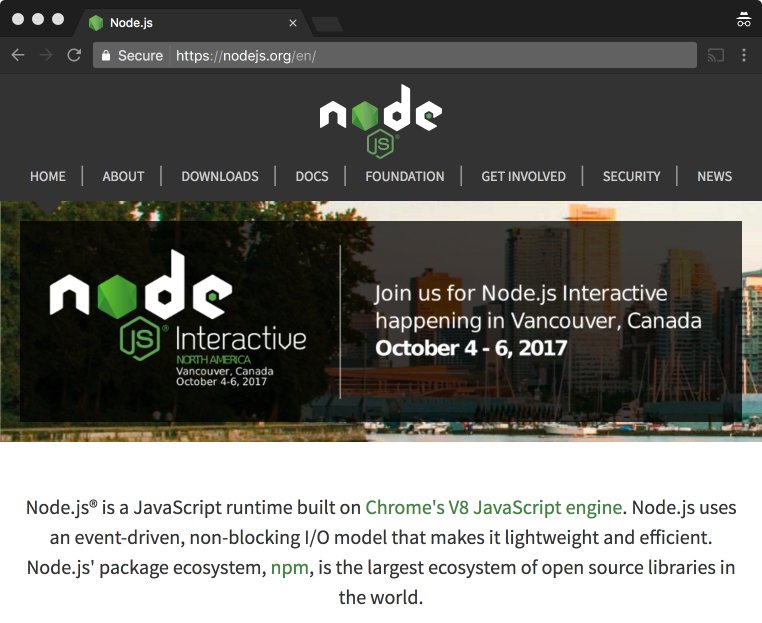
\includegraphics[width=\textwidth]{screenshot.png}
  \caption{A screenshot.}
  \label{figure:example}
\end{figure}
  \chapter{Conclusion}
\label{chapter:conclusion}
  
The report concludes here.
  \newpage
  % Include the bibliography.
  \bibliographystyle{plain}
  \bibliography{bibliography}

\end{document}